% Source: graduate-coursework/Research/How_to_write/00_Contrastive_Synthesis.tex
% Description: \textbf{Post-Process Theory (Kent, 1993, 1999).

\documentclass[border=4pt]{standalone}
\usepackage{newtxtext,newtxmath}
\usepackage{tikz}
\usetikzlibrary{arrows.meta,positioning,shapes.geometric,calc,decorations.pathreplacing}

\definecolor{garnet}{HTML}{73000A}
\definecolor{atlantic}{HTML}{466A9F}
\definecolor{congaree}{HTML}{1F414D}
\definecolor{horseshoe}{HTML}{65780B}
\definecolor{rose}{HTML}{CC2E40}
\definecolor{honeycomb}{HTML}{A49137}
\definecolor{warmgrey}{HTML}{676156}
\definecolor{black90}{HTML}{363636}
\definecolor{black70}{HTML}{5C5C5C}
\definecolor{black50}{HTML}{A2A2A2}
\definecolor{black30}{HTML}{C7C7C7}
\definecolor{black10}{HTML}{ECECEC}
\definecolor{sandstorm}{HTML}{FFF2E3}

\begin{document}
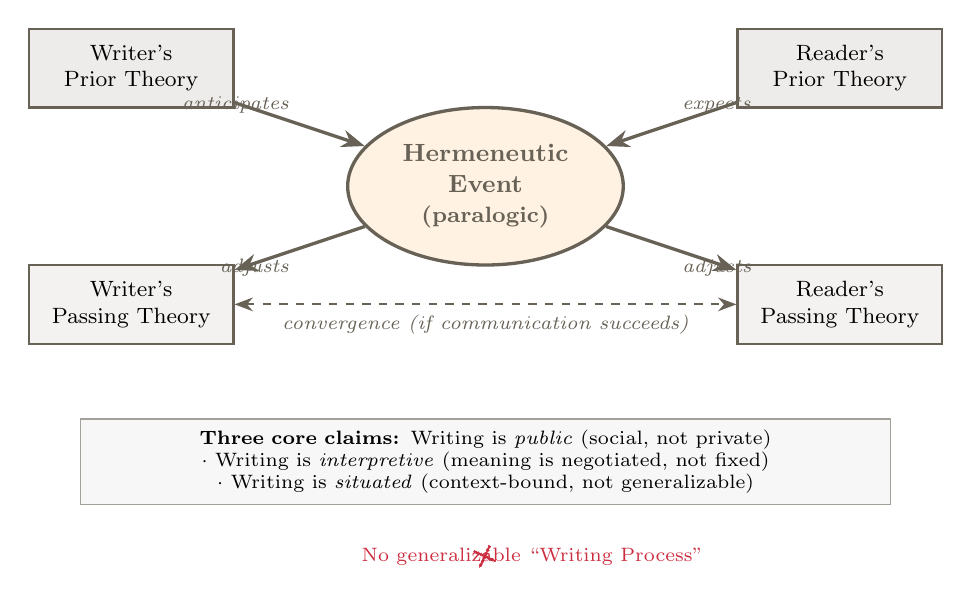
\begin{tikzpicture}[
    every node/.style={font=\footnotesize},
    box/.style={rectangle, draw=warmgrey, thick, fill=warmgrey!8,
        minimum width=2.6cm, minimum height=1cm, align=center, font=\footnotesize},
]

% Writer side
\node[box, fill=warmgrey!12] (wprior) at (-4.5, 2) {Writer's\\Prior Theory};
\node[box] (wpassing) at (-4.5, -1) {Writer's\\Passing Theory};

% Reader side
\node[box, fill=warmgrey!12] (rprior) at (4.5, 2) {Reader's\\Prior Theory};
\node[box] (rpassing) at (4.5, -1) {Reader's\\Passing Theory};

% Central hermeneutic event
\node[ellipse, draw=warmgrey, very thick, fill=sandstorm,
    minimum width=3.5cm, minimum height=2cm, align=center,
    font=\small\bfseries, text=warmgrey] (event) at (0, 0.5) {Hermeneutic\\Event\\{\footnotesize (paralogic)}};

% Arrows from prior to passing through event
\draw[-{Stealth}, very thick, warmgrey] (wprior) -- (event)
    node[midway, above left, font=\scriptsize\itshape] {anticipates};
\draw[-{Stealth}, very thick, warmgrey] (rprior) -- (event)
    node[midway, above right, font=\scriptsize\itshape] {expects};
\draw[-{Stealth}, very thick, warmgrey] (event) -- (wpassing)
    node[midway, below left, font=\scriptsize\itshape] {adjusts};
\draw[-{Stealth}, very thick, warmgrey] (event) -- (rpassing)
    node[midway, below right, font=\scriptsize\itshape] {adjusts};

% Convergence zone
\draw[{Stealth}-{Stealth}, thick, warmgrey, dashed] (wpassing) -- (rpassing)
    node[midway, below, font=\scriptsize\itshape] {convergence (if communication succeeds)};

% Three core claims
\node[rectangle, draw=warmgrey!60, fill=warmgrey!5, inner sep=4pt,
    font=\scriptsize, align=center, text width=10cm] at (0, -3)
    {\textbf{Three core claims:} Writing is \textit{public} (social, not private) $\cdot$
    Writing is \textit{interpretive} (meaning is negotiated, not fixed) $\cdot$
    Writing is \textit{situated} (context-bound, not generalizable)};

% X through "Process" label
\node[font=\large, text=rose, rotate=20] at (0, -4.2) {\sffamily\bfseries \texttimes};
\node[font=\scriptsize, text=rose] at (0.6, -4.2) {No generalizable ``Writing Process''};

\end{tikzpicture}
\end{document}
